\documentclass[20pt,landscape,dvips]{foils} 
% add 'draft' option above to exclude image when compiling
\usepackage[french]{babel}
\usepackage[utf8]{inputenc}  
\usepackage{csquotes} 
%\MakeOuterQuote{"}
\frenchspacing
\DecimalMathComma

\usepackage{latexsym}
\usepackage{amsmath,amssymb,amsfonts}
\usepackage{MnSymbol}
\usepackage{url}
\usepackage{graphicx}
%\usepackage[dvipsnames]{xcolor}
\usepackage{hyperref}
\usepackage{alltt}
\usepackage{pifont,manfnt}
\usepackage[dvipsnames,table]{xcolor}
\usepackage{subfig}
%\usepackage{enumerate}
%\usepackage{colortbl}
\usepackage{multirow,hhline}
\usepackage{cclicenses}
\setlength\parindent{0pt}
\hypersetup{colorlinks=true,citecolor=black,urlcolor=black,linkcolor=black}
\usepackage[style=verbose]{biblatex}
\bibliography{refs}

\newcommand{\highlight}[1]{\textcolor{Plum}{\bfseries #1}}
\newcommand{\remark}[1]{%
%\centerline{
\begin{center}
\framebox[.9\textwidth][t]{
\ding{46} 
\parbox[t]{.8\textwidth}{\small #1}}
\end{center}}

\DeclareMathOperator*{\inlaw}{\sim}
\newcommand{\iid}{\inlaw_{\text{i.i.d.}}}
%\newcommand{\iid}{\mathop{\mathrm{diag}}}
\newcommand{\pobs}{p_{\text{obs}}}

\reversemarginpar
\def\mark{\marginpar{\dbend}}

%\newcommand{\bm}[1]{\mbox{\boldmath{$#1$}}}
\renewcommand{\abstractname}{Summary}
\newcommand\bs{\char '134}   %  a backslash character for the \tt font
%\renewcommand\refname{Additional Readings}

% customize header/footer
\rightheader{}
% Note about the copyleft symbol:
% I use a custom reversed and circled "c" char because \textcopyleft in
% the textcomp package does not support sans serif font.
% Also, "c" is shifted horizontally by 1ex to align with the circle.
%\Restriction{\mbox{\raisebox{1.5ex}{\rotatebox{180}{\textcircled{c\kern.1ex}}} 2009}, \url{www.aliquote.org}}
% now I use the CC licence...
% \Restriction{\cc 2016 \VCRevision}
\Restriction{\cc 2016 Module 11 EESPE}

\title{Méthodes psychométriques en qualité de vie}
\author{Christophe Lalanne\\EA 7334 REMES\\ Unité de Méthodologie des critères d’évaluation\\Université Paris-Diderot, Sorbonne Paris-Cité\\}
\date{
\includegraphics[height=18ex]{logo.eps}}

%%% This file has been generated by the vc bundle for TeX.
%%% Do not edit this file!
%%%
%%% Define Git specific macros.
\gdef\GITHash{f4328f7906d309e9224e3e5c2f7f36477f44e69f}%
\gdef\GITAbrHash{f4328f7}%
\gdef\GITParentHashes{136657e4877819e72dc9ebb2f209631a2a8d1057}%
\gdef\GITAbrParentHashes{136657e}%
\gdef\GITAuthorName{Christophe Lalanne}%
\gdef\GITAuthorEmail{ch.lalanne@gmail.com}%
\gdef\GITAuthorDate{2016-07-06 10:29:58 +0200}%
\gdef\GITCommitterName{Christophe Lalanne}%
\gdef\GITCommitterEmail{ch.lalanne@gmail.com}%
\gdef\GITCommitterDate{2016-07-06 10:29:58 +0200}%
%%% Define generic version control macros.
\gdef\VCRevision{\GITAbrHash}%
\gdef\VCAuthor{\GITAuthorName}%
\gdef\VCDateRAW{2016-07-06}%
\gdef\VCDateISO{2016-07-06}%
\gdef\VCDateTEX{2016/07/06}%
\gdef\VCTime{10:29:58 +0200}%
\gdef\VCModifiedText{\textcolor{red}{with local modifications!}}%
%%% Assume clean working copy.
\gdef\VCModified{0}%
\gdef\VCRevisionMod{\VCRevision}%


\begin{document}
\LogoOff
\maketitle
\rightfooter{\quad\textsf{\thepage}}



%---------------------------------------------------------------Slide-
\foilhead{Fidélité de mesure}
\begin{itemize}
\item Consistance interne d'une échelle
\item Accord inter-juges (cas binaire ou non)
\item Corrélation intra-classe
\end{itemize}



% ---------------------------------------------------------------Slide-
\foilhead{Comment évaluer la fidélité de mesure}

Une formulation alternative consiste à se demander quelles sont les sources
potentielles de variation des scores, et donc comment les mesurer et quel est
leur impact lorsque l'on infère des résultats observés sur un échantillon à la
population ?

Des mesures collectées plusieurs fois à partir d'un même instrument peuvent
survenir de plusieurs manières\autocite{Dunn2000} :
\begin{itemize}
\item évaluation répétée de plusieurs sujets par le même évaluateur ;
\item évaluation alternative d'un même individu par plusieurs évaluateurs ;
\item administration répétée d'un même questionnaire ; 
\item utilisation de différentes sous-échelles d'un même questionnaire.
\end{itemize}

% ---------------------------------------------------------------Slide-
\foilhead{Outils statistiques}

La fidélité ou précision de mesure peut être quantifiée à l'aide de différentes
techniques :
\begin{itemize}
\item \highlight{décomposition (linéaire) des composantes de variance en TCT} ;
\item modèles d'équations structurelles ;
\item modèles de réponse à l'item.
\end{itemize}
\medskip

L'objectif des études de fidélité est de quantifier le degré de précision d'une
mesure afin de justifier les qualités métrologiques de l'instrument de mesure
(reproductibilité des scores, comparaisons inter-groupes, etc.). 


% ---------------------------------------------------------------Slide-
\foilhead{Fidélité de mesure $\neq$ significativité}

La \highlight{significativité statistique} est utilisée pour évaluer la
probabilité ou la vraisemblance de résultats observés sur un échantillon en
référence à un modèle de population sous l'hypothèse nulle ; la
\highlight{significativité pratique ou clinique} reflète le degré de divergence
des résultats observés avec l'hypothèse nulle (tel que mesuré par une mesure de
taille d'effet) -- sous laquelle on ne distingue pas les patients des sujets
contrôles\autocite{Thompson2003}.

Mais ces deux concepts supposent que les scores sur lesquelles les conclusions
reposent sont des indicateurs corrects et précis de la performance ou de l'état
mesuré chez l'individu.

% ---------------------------------------------------------------Slide-
\foilhead{}

\begin{quote}
It is important to remember that a test is not reliable or
unreliable. Reliability is a property of the scores on a test for a
particular population of examinees (Feldt~\& Brennan, 1989). Thus,
authors should provide reliability coefficients of the scores for the
data being analyzed even when the focus of their research is not
psychometric.

\raggedleft Wilkinson \& APA Task Force\autocite{Wilkinson1999}
\end{quote}


%---------------------------------------------------------------Slide-
\foilhead{Modèle de mesure}
\hfill $\triangleright$ 01a-scores.pdf

Pour un individu $i$ évalué sur une seule occasion, son score $x_i$ peut être
exprimé comme suit : 
\[
\textcolor{CornflowerBlue}{x_i} = \textcolor{Apricot}{\tau_i} +
\textcolor{Thistle}{\varepsilon_i},\quad \varepsilon_i\sim\mathcal{N}(0;\sigma_e^2),
\]
d'où l'on en déduit naturellement que $\mathbb{E}(X)=T$ (\enquote{par construction}).

Si l'on suppose que $T$ et $E$ sont indépendants, on a également
\[
\mathbb{V}(X) = \mathbb{V}(T)+\mathbb{V}(E)
\]

% ---------------------------------------------------------------Slide-
\foilhead{}
On peut définir le \highlight{coefficient de fidélité} de la manière suivante :
\begin{eqnarray}\label{eq:rx}
  R_X & = & \frac{\mathbb{V}(T)}{\mathbb{V}(X)}\nonumber\\
      & = & \frac{\mathbb{V}(T)}{\mathbb{V}(T)+\mathbb{V}(E)}.
\end{eqnarray}

Il s'agit d'une variable aléatoire donc ce n'est pas une propriété fixe d'un
instrument de mesure. La racine carré de ce coefficient est appelée
\highlight{erreur standard de mesure} (SEM).

% ---------------------------------------------------------------Slide-
\foilhead{Extension simple de ce modèle de mesure}
Supposons que les évaluations ne dépendent pas seulement du score vrai des
individus mais également de l'évaluateur (les effets étant supposés
indépendants).

Si tous les sujets sont évalués par le même évaluateur, $R_X$ se calcule tel que
défini en~(\ref{eq:rx}). Si, au contraire, les individus sont évalués par des
évaluateurs choisis aléatoirement , alors
\begin{equation}\label{eq:rxprime}
    R'_X=\frac{\mathbb{V}(T)}{\mathbb{V}(T)+\mathbb{V}(I)+\mathbb{V}(E)},
\end{equation}
et $R_X^{}>R'_X$.

% ---------------------------------------------------------------Slide-
\foilhead{Le cas de deux instruments}
Supposons que nous disposons d'une série de données appariées collectées à
partir de deux instruments de mesure, $\mathcal{I}_X$ et $\mathcal{I}_Y$, pour
lesquels les scores sont construits selon le même schéma :
\begin{eqnarray*}
	X & = & T_X+E_X\\
	Y & = & T_Y+E_Y\\
\end{eqnarray*}
Quelle est la corrélation entre $X$ et $Y$ ?

Les\mark{} deux séries de mesure sont des réalisations des variables alétoires
$X$ et $Y$, mais la précision des instruments de mesure entre également en jeu.

% ---------------------------------------------------------------Slide-
\foilhead{Corrélation atténuée}

La corrélation (liénaire) entre $X$ et $Y$ est donnée par
$\rho_{XY}=\frac{\text{cov}(T_X,T_Y)}{\sqrt{\mathbb{V}(T_X)\mathbb{V}(T_Y)}}$.
Un bon estimateur peut être consrtuit comme suit :
\begin{eqnarray}\label{eq:corr}
	\hat\rho_{XY} & = & \frac{\text{cov}(X,Y)}{\sqrt{\mathbb{V}(X)\mathbb{V}(Y)}}\nonumber\\
	              & = &
                      \frac{\text{cov}(T_X+E_X,T_Y+E_Y)}{\sqrt{\mathbb{V}(T_X+E_X)\mathbb{V}(T_Y+E_Y)}}
                  =\rho_{XY}\sqrt{R_XR_Y}
\end{eqnarray}

La corrélation entre les données observées est atténuée par la précision de
chacun des instruments de mesure.

% ---------------------------------------------------------------Slide-
\foilhead{}
Il en va de même dans le cas de la régression linéaire : si l'on souhaite
prédire $Y$ à partir de $X$ à l'aide d'un modèle de régression simple,
$\mathbb{E}(T_Y|T_X)=\beta_0+\beta_1T_X$, la pente serait estimée par
$\beta_1=\text{cov}(T_X,T_Y)/\mathbb{V}(T_X)$. En tenant compte de la précision de
la mesure $X$, $R_X$, on considèrera comme estimateur :
\begin{eqnarray}\label{eq:slope}
	\hat\beta_1 & = & \frac{\text{cov}(X,Y)}{\mathbb{V}(X)}\nonumber\\          
              & = & \frac{R_X\text{cov}(T_X,T_Y)}{\mathbb{V}(T_X)}=R_X\beta_1
\end{eqnarray}

La pente de la droite de régression est atténuée (c.a.d. ramenée vers 0).

% ---------------------------------------------------------------Slide-
\foilhead{Consistance interne d'un instrument}

La consistance interne d'un questionnaire permet de résumer le degré
d'homogénéité des scores aux items (variance partagée avec le score
total).

La \highlight{consistance interne} est considérée comme une borne basse de la fidélité de
mesure, et elle est souvent mesurée à l'aide du \highlight{coefficient alpha de
  Cronbach}, qui est une mesure dépendant de l'échantillon. Lorsque $\alpha =
0,70$, l'erreur de mesure vaut environ 0,55 $\times$ l'écart-type du score
total.

Un tel indicateur suppose l'absence de corrélation entre les erreurs de mesure,
une contribution équivalente des items dans la détermination du score total, et
l'unidimensionalité de l'instrument de mesure.

L'\highlight{erreur de mesure} se calcule comme $\sigma_e =
\sigma\sqrt{1-\alpha}$, où $\sigma^2$ désigne la variance des scores totaux.

% ---------------------------------------------------------------Slide-
\foilhead{Indice KR-20 et alpha de Cronbach}
Dans le cas des items dichotomiques, une mesure de consistance est le
coefficient de Kuder-Richardson (KR-20) \autocite{kuder37}:
\begin{equation}
\text{KR-20}=\frac{K}{K-1}\left[1-\frac{\sum_k p_kq_k}{\sigma^2}\right]
\end{equation}
où $K$ est le nombre d'items, $\sigma^2$ la variance des scores totaux, $p_k$
et $q_k$ désignent les proportions d'individus avec un score à 1 ou 0 à l'item
$k$. 

Dans le cas des items polytomiques, on remplacera $p_kq_k$ par
$\sigma_k^2$, la variance des scores à l'item $k$ \autocite{cronbach51}.

% ---------------------------------------------------------------Slide-
\foilhead{Intérêts et limites}

\begin{quote}
Coefficients are a crude device that does not bring to the surface
many subtleties implied by variance components. In particular, the
interpretations being made in current assessments are best evaluated
through use of a standard error of measurement\autocite{Cronbach2004}.
\end{quote}

\begin{itemize}
\item L'alpha de Cronbach n'est pas une mesure de
  l'unidimensionalité\autocite{danes84} ;
\item L'alpha de Cronbach, comme toute estimation de fidélité de mesure des
  scores, dépend de l'échantillon ; il dépend également du nombre d'items.
\end{itemize}

% ---------------------------------------------------------------Slide-
\foilhead{}

Pour une taille d'échantillon fixe ($N=300$), l'alpha de Cronbach augmente de
manière monotone avec le nombre d'items inclus dans l'échelle ou le degré
d'intercorrélation ($\rho$) entre les items. Avec 30 items et $\rho=0.350$, on
peut obtenir $\alpha=0.943$ ($\alpha=0.910$ avec 20 items).

Alternatives au coefficient $\alpha$ :
\begin{itemize}
\item Guttman Lambda 6 (part de variance de chaque item expliquée par la
  régression de l'ensemble des autres items, ou plus exactement la variance des
  erreurs) ;
\item Revelle beta, McDonald omega, Sijtma GLB, etc.\autocite{zinbarg05}
\end{itemize}

% ---------------------------------------------------------------Slide-
\foilhead{Illustration}

Cas d'un instrument avec 4 items, ayant la même erreur de mesure ($0,36$):
\begin{alltt}
library(psych)
set.seed(101)
\textcolor{Apricot}{x} <- sim.congeneric(loads = rep(\highlight{0.8}, \highlight{4}), \hfill\ding{182} \ding{183}
                    N = 100, short = FALSE)
\end{alltt}


\begin{alltt}\small
> alpha(x$observed)

Reliability analysis
Call: alpha(x = x$observed)

  raw_alpha std.alpha G6(smc) average_r S/N  ase   mean  sd
      0.88      0.88    0.84      0.64 7.1 0.02 -0.071 0.8

 lower alpha upper     95% confidence boundaries
0.84 0.88 0.92

 Reliability if an item is dropped:
   raw_alpha std.alpha G6(smc) average_r S/N alpha se
V1      0.82      0.82    0.76      0.60 4.6    0.031
V2      0.84      0.84    0.78      0.63 5.1    0.028
V3      0.85      0.85    0.80      0.66 5.9    0.025
V4      0.86      0.86    0.80      0.67 6.0    0.025
\end{alltt}
%$$$

% ---------------------------------------------------------------Slide-
\foilhead{Fidélité inter-cotateur}

Le coefficient Kappa de Cohen est utilisé pour évaluer la concordance dans le
cas de deux évaluations (supposées indépendantes) permettant de classer un
individu selon un critère binaire\autocite{cohen60} (p.ex., radio pulmonaire
pour la tuberculose) ou d'attribuer un score numérique à un
individu\autocite{cohen68} (p.ex., sévérité du trouble psychiatrique).
\begin{equation}
  \kappa=\frac{\overbrace{\sum_i\pi_{ii}}^{\textrm{\footnotesize raw agreement}}\hskip-2ex-\sum_i\pi_{i\bullet}\pi_{\bullet
      i}}{1-\hskip-1ex\underbrace{\sum_i\pi_{i\bullet}\pi_{\bullet i}}_{\textrm{\footnotesize random ratings}}}
\end{equation}


% ---------------------------------------------------------------Slide-
\foilhead{}
Le coefficient $\kappa$ est asymptotiquement équivalent à l'ICC estimé à partir
d'une ANOVA à deux effets aléatoires, même si les tests de significativité et
les intervalles de confiance ne sont pas adaptés au cas binaire. 

Il existe des extensions pour le cas où il y a plus de 2
cotateurs\autocite{siegel88}, ainsi que des règles d'interprétation des valeurs
de $\kappa$\autocite{fleiss81b}.

% ---------------------------------------------------------------Slide-
\foilhead{Concordance inter-juges et études diagnostiques}

Exemple d'un diagnostique (malade/pas malade) fourni par deux
psychiatres\autocite{dunn00} :
\begin{center}
\small
\begin{tabular}{l|l|cc|c|}
\multicolumn{2}{c}{}& \multicolumn{2}{c}{$A$} & \multicolumn{1}{c}{}\\
\cline{3-5}
\multicolumn{2}{c|}{}& Case & Non-case & Total\\
\cline{2-5}
\multirow{2}{*}{$B$} & Case & $p_{11}$ & $p_{12}$ & $p_{1\bullet}$\\
& Non-case & $p_{21}$ & $p_{22}$ & $p_{2\bullet}$\\
\cline{2-5}
& Total & $p_{\bullet 1}$ & $p_{\bullet 2}$ & 1\\
\cline{2-5}
\end{tabular}
\end{center}
\medskip

La concordance brute vaut $P_o=p_{11}+p_{22}$ et le taux attendu sous
l'hypothèse d'un jugement au hasard $P_c=p_{1\bullet}p_{\bullet
  1}+p_{2\bullet}p_{\bullet 2}$. \newline
On a donc : $\kappa=(P_o-P_c) / (1-P_c)$.



% ---------------------------------------------------------------Slide-
\foilhead{Illustration}

Cas de l'évaluation de 118 tumeurs sur une échelle en 5 points\autocite{agresti90} :
\begin{alltt}
data(pathologist.dat, package = "exactLoglinTest")
aa <- xtabs(y ~ A + B, data = pathologist.dat)
\end{alltt}
\begin{alltt}\small
> aa
   B
A    1  2  3  4  5
  1 \highlight{22}  \textcolor{CornflowerBlue}{5}  0  0  0
  2  \textcolor{CornflowerBlue}{2}  \highlight{7}  \textcolor{CornflowerBlue}{2}  1  0
  3  2 \textcolor{CornflowerBlue}{14} \highlight{36} \textcolor{CornflowerBlue}{14}  3
  4  0  0  \textcolor{CornflowerBlue}{0}  \highlight{7}  \textcolor{CornflowerBlue}{0}
  5  0  0  0  \textcolor{CornflowerBlue}{0}  \highlight{3}
> sum(diag(aa))/sum(aa)  \hfill\ding{182}
[1] 0.6355932
> cohen.kappa(aa)
Call: cohen.kappa1(x = x, w = w, n.obs = n.obs, alpha = alpha)

Cohen Kappa and Weighted Kappa correlation coefficients and confidence boundaries
                 lower estimate upper
unweighted kappa  0.39     0.50  0.61
weighted kappa    0.70     0.78  0.86  \hfill\ding{183}

 Number of subjects = 118
\end{alltt}


% ---------------------------------------------------------------Slide-
\foilhead{Autres mesures d'association}

Les coefficients de \highlight{corrélation tétrachorique} (cas binaire) et
\highlight{polychorique} (cas ordinal) peuvent être utilisés comme mesure de
concordance entre juges.

En effet, ils permettent
\begin{itemize}
\item d'estimer l'association entre les deux évaluations si celles-ci étaient
  réalisées sur une \textcolor{CornflowerBlue}{échelle continue} ;
\item de tester l'homogénéité marginale entre les juges.
\end{itemize}
\medskip

Dans ce cas, on se rapproche des modèles en traits latents \autocite{uebersaxA},
avec des hypothèses spécifiques sur les distributions.

% ---------------------------------------------------------------Slide-
\foilhead{Cas de la corrélation tétrachorique}

\begin{minipage}{0.45\textwidth}
\centerline{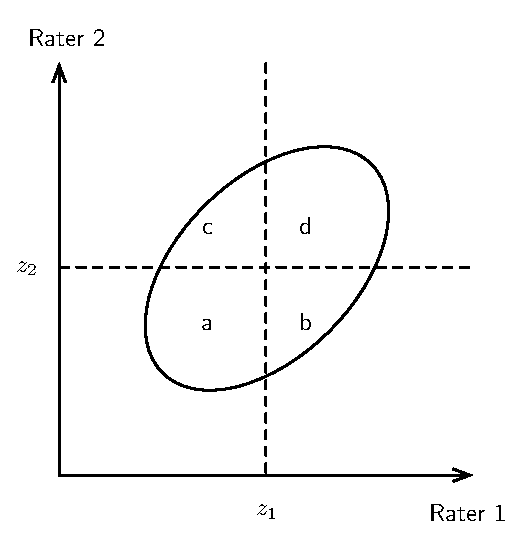
\includegraphics[scale=.85]{./figs/tetrachoric.eps}}
\end{minipage}\hfill
\begin{minipage}{0.5\textwidth}
	\small
La figure de gauche représente graphiquement le tableau croisé de deux
évaluations :
\vspace*{.5cm}

\begin{tabular}{lc|c|c|c}
& \multicolumn{1}{c}{} &	\multicolumn{2}{c}{Rater 1} & \\
& \multicolumn{1}{c}{} & \multicolumn{1}{c}{$-$} & \multicolumn{1}{c}{$+$} & \\
\cline{3-4}
\multirow{2}{*}{Rater 2} & $-$ & $a$ & $b$ & $a+b$ \\
\cline{3-4}
& $+$ & $c$ & $d$ & $c+d$ \\
\cline{3-4}
& \multicolumn{1}{c}{} & \multicolumn{1}{c}{$a+c$} & \multicolumn{1}{c}{$b+d$} & 1 \\
\end{tabular}
\end{minipage}

Ici $a=\Pr(Y_1<z_1\;\text{et}\;Y_2<z_2)$ est la fonction de répartition d'une
distribution binormale, c.a.d. $\displaystyle
\int_{-\infty}^{z_2}\int_{-\infty}^{z_1}\Phi(x,y,r)dxdy$, où $\Phi(\bullet)$ est
la fonction de densité d'une loi binormale, avec $\Phi(z_1) = a+c$ et $\Phi(z_2)
= a+b$ (valeurs seuil).


% ---------------------------------------------------------------Slide-
\foilhead{Illustration : plusieurs cotateurs}

Cas de l'évaluation de 7 experts sur une échelle en 100 points portant sur 8
approches permettant de résumer la qualité de vie\autocite{hays05}.

\begin{center}
\footnotesize
\begin{tabular}{lrrrrrrrrr}
  \hline
  Approach & \multicolumn{7}{l}{Rater} & Mean & SD\\
  \cline{2-8}
  & 1 & 2 & 3 & 4 & 5 & 6 & 7 & & \\
  \hline
  1 & 90 & 00 & 50 & 95 & 30 & 60 & 50 & 53.57 & 33.00\\
  2 & 90 & 00 & 70 & 100 & 60 & 55 & 80 & 65.00 & 32.79\\
  3 & 90 & 51 & 40 & 90 & 25 & 100 & 85 & 68.71 & 29.44\\
  4 & 30 & 52 & 05 & 30 & -- & 10 & 40 & 27.93 & 17.78\\
  5 & 80 & 50 & 80 & 60 & 80 & 50 & 100 & 71.43 & 18.64\\
  6 & 30 & 100 & 05 & 50 & 50 & 40 & 40 & 45.00 & 28.72\\
  7 & 20 & 70 & 00 & 20 & 10 & 00 & 01 & 17.29 & 24.86\\
  8 & 20 & 90 & 00 & 00 & 00 & 00 & 01 & 16.57 & 33.18\\
  \hline
\end{tabular}
\end{center}

%---------------------------------------------------------------Slide-
\foilhead{}
\begin{minipage}{0.45\textwidth}
\centerline{\includegraphics[scale=.85]{./figs/hays05.eps}}
\end{minipage}\hfill
\begin{minipage}{0.5\textwidth}
\small
Médiane $\pm$ IQR (figure de gauche).\\
Les approches considérées comme les plus adéquates (scores plus élevés) sont
associées à une plus grande variabilité entre juges même si la corrélation de
rang (Spearman) entre la moyenne et l'écart-type n'est pas significative
($\rho=-0,167,\, p=0,703$). 
\end{minipage}

%---------------------------------------------------------------Slide-
\foilhead{Analyse des composantes de variance}

Les commandes R suivantes permettent d'estimer un modèle à un facteur (effet
fixe) \ding{182}, un modèle à deux effets \ding{183}, et un modèle mixte
incluant deux effets \ding{185}. 

\begin{alltt}
load("hays05.rda")
require(lme4)
summary(aov(score ~ approach, hays05)) \hfill\ding{182}
summary(aov(score ~ rater+approach, hays05)) \hfill\ding{183}
summary(aov(score ~ approach*rater, hays05)) \hfill\ding{184}
summary(lmer(score ~ approach + (1 | rater), hays05)) \hfill\ding{185}
\end{alltt}

Le modèle~\ding{183} est largement utilisé en pratique et permet d'estimer l'ICC
dit de consistence ou de condordance \autocite{shrout79}. 

%---------------------------------------------------------------Slide-
\foilhead{}

\begin{center}
\small
\begin{tabular}{lrrl}
  \cline{1-3}
  Source & Df & MS & \\ 
  \cline{1-3}
  Approach         & 7 & 3597.8 & \multirow{2}{*}{$\Big\rbrace$~\ding{182}}\\ 
  Within              & 47 & 792.6 & \\
  Rater                & 6 & 844.7  & \multirow{2}{*}{$\Big\rbrace$~\ding{184}}\\ 
  Approach$\times$Rater & 41 & 785.0 & \\ 
  Total                & 54 & &\\
   \cline{1-3}
\end{tabular}
\end{center}

\begin{center}
\small
\begin{tabular}{ccc}
\hline
Model & Reliability & ICC\\
\hline
\ding{182} &
$\frac{\textrm{MS}_{B}-\textrm{MS}_{W}}{\textrm{MS}_{B}}$ &
$\frac{\textrm{MS}_{B}-\textrm{MS}_{W}}{\textrm{MS}_{B}+(K-1)\textrm{MS}_{W}}$ \\[10pt]
\ding{183} & $\frac{\textrm{MS}_{B}-\textrm{MS}_{E}}{\textrm{MS}_{B}}$ &
$\frac{\textrm{MS}_{B}-\textrm{MS}_{E}}{\textrm{MS}_{B}+(K-1)\textrm{MS}_{E}}$
\\[10pt]
\ding{184} &
$\frac{N(\textrm{MS}_{B}-\textrm{MS}_{E})}{N\textrm{MS}_{B}+\textrm{MS}_{J}-\textrm{MS}_{E}}$ & 
$\frac{\textrm{MS}_{B}-\textrm{MS}_{E}}{\textrm{MS}_{B}+(K-1)\textrm{MS}_{E}+K(\textrm{MS}_{J}-\textrm{MS}_{E})/N}$
\\[10pt]
\hline
\end{tabular}
{\par\scriptsize MS, mean square for between-subject ($B$),
  within-subject ($W$) effects; $K$, number of replications; $N$,
  number of ratees.}
\end{center}

% ---------------------------------------------------------------Slide-
\foilhead{}

Fichier de données et scripts R disponibles à l'adresse suivante :\newline
{\centering \url{https://bitbucket.org/chlalanne/eespe11}\par}
\vfill

\raggedleft \scriptsize -- Typeset with \FoilTeX\ (version 2), Revision \VCRevision

\end{document}
